\documentclass[11pt,a4paper]{article} 
\usepackage{amssymb}
\usepackage[shortlabels]{enumitem}
\usepackage[fleqn]{amsmath} 
\usepackage{relsize}
\usepackage{graphicx}
\usepackage[super]{nth}
\usepackage{hyperref, url}
\usepackage[margin=2cm, top=2cm]{geometry}
\graphicspath{{./img/}}
\newcommand\setItemNumber[1]{\setcounter{enumi}{\numexpr#1-1\relax}}
\newcommand*{\mybox}[1]{\framebox{#1}}
\newcommand{\tuple}[1]{$\langle #1 \rangle$} 
\newcommand{\stuple}[1]{$\langle$#1$\rangle$} % ordered pair with strings inside
\newcommand{\forceindent}{\leavevmode{\parindent=1em\indent}}
\DeclareUnicodeCharacter{2212}{-}
\title{\bf Homework 8\\[1ex]
\rm\normalsize CS250 Discrete Structures I, Winter 2020 }
\date{\normalsize Due: May, 27, 2020}
\author{\normalsize Armant Touche}

\begin{document} 
\vspace{0cm}\maketitle 
	
	
	\subparagraph{Problem 1} 4.1 Graph Definitions (pg. 243-246) \\
			
		From section 4.1 in the textbook, complete exercises 1, 3, 7, 8, 12, 13

        \begin{enumerate}

        %1
        \item  If 10 people each shake hands with each other, how many handshakes took place? What does this question have to do with graph theory?\\
            Using the Handshake Lemma and dividing the sum by two since the sum of degrees counts each edge twice, I am able to compute the number of handshake between 10 people by using
            $$ (\sum_{v\in V} d(10)) = 90\div 2 = 45\;\;\text{(handshakes)}$$

        %3
        \setItemNumber{3}
    \item Is it possible for two \textit{different} (non-isomorphic) graphs to have the same number of vertices and the same number of edges? What if the degrees of the vertices in the two graphs are the same (so both graphs have vertices with degrees 1, 2, 2, 3, and 4, for example)? Draw two such graphs or explain why not.\\\\
        Notice the picture below, $G_1 \ncong G_2$ but $V_1\cong V_2$  

            \begin{center}
            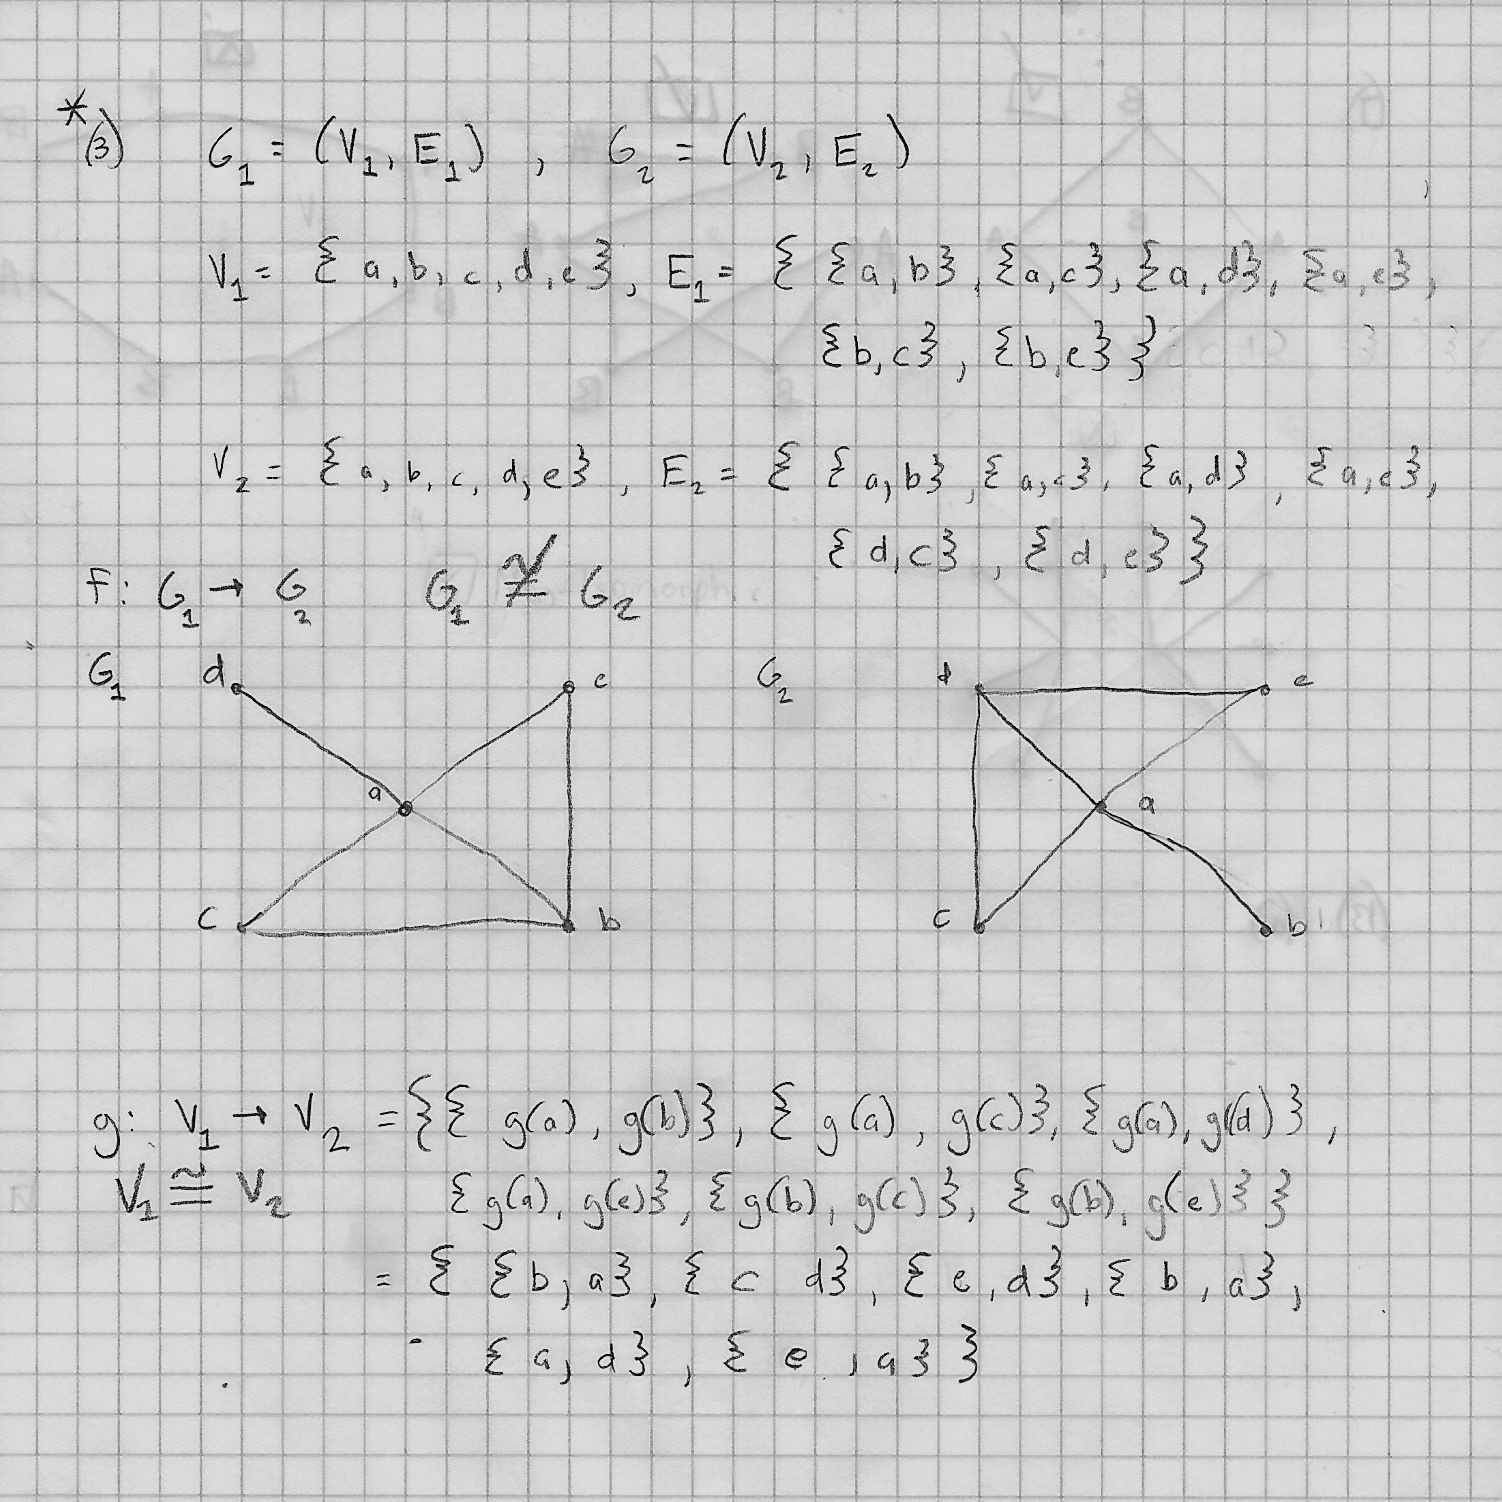
\includegraphics[width=.60\textwidth]{hw8_graphic3}
            \end{center}

        \newpage
        %7
        \setItemNumber{7}
        \item Which of the graphs below are bipartite? Justify your answers

            \begin{center}
            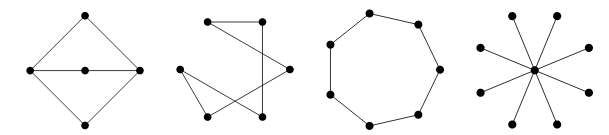
\includegraphics[width=.5\textwidth]{hw8_graphic1}
            \end{center}

            \begin{center}
            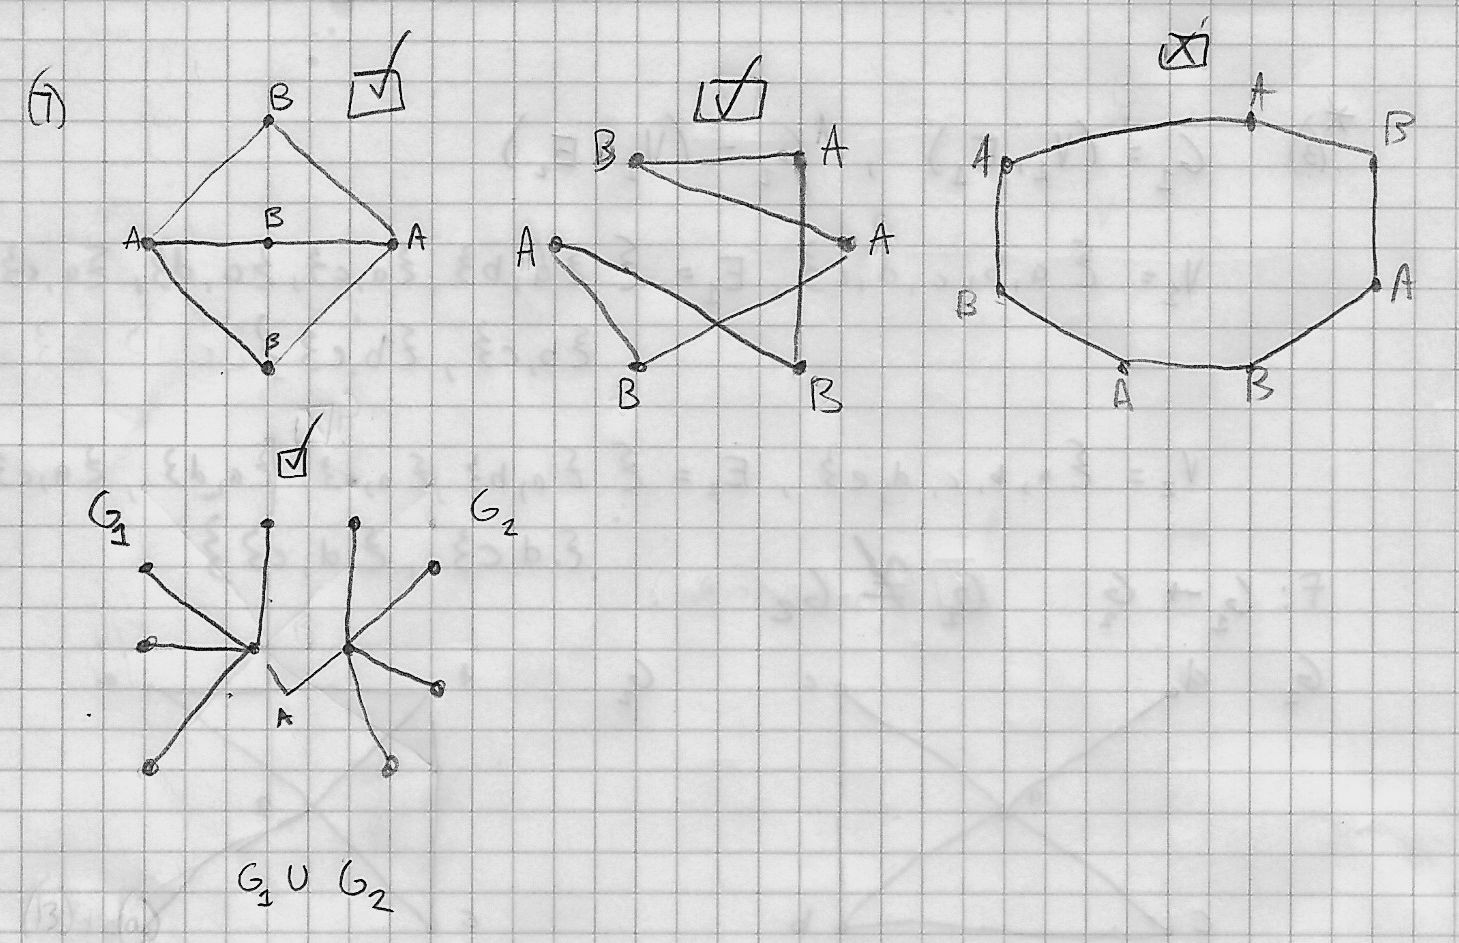
\includegraphics[width=.5\textwidth]{hw8_graphic4}
            \end{center}


        %8
        \item For which $n\geq 3$ is the graph $C_n$ bipartite?\\
            $C_n$ is bipartite such that when $n$ is an even integer.

        %12
        \setItemNumber{12}
    \item We often define graph theory concepts using set theory. For example, given a graph $G = (V, E)$ and a vertex $v\in V$, we define
        $$N(v) = \{u\;\in V\; |\; \{v,u\}\;\in E\}$$
        We define $N[v] = N(v)\cup \{v\}$. The goal of this problem is to figure out what all this means.
        \begin{enumerate}

        \item Let $G$ be the graph with $V = \{a,b,c,d,e,f\}$ and\\ $E = \{\{a,b\},\{a,e\},\{b,c\},\{b,e\},\{c,d\},\{c,f\},\{d,f\},\{e,f\}\}$. \\Find $N(a)$, $N[a]$, $N(c)$, and $N[c]$.\\
            $N(a) = \{ \{a,b\}, \{a,e\}\}\\ N[a] = N(a)\cup \{a\}\\ = \{\emptyset,\{a\},\{a,b\},\{a,e\}\}$\\
            $N(c) = \{\{c,d\},\{c,f\}\}\\N[c] = N(c)\cup\{c\}\\ = \{\emptyset,\{c\}, \{b,c\},\{c,d\},\{c,f\}\}$
        \item What is the largest and smallest possible values for $|N(v)|$ and $|N[v]|$ for the graph in part (a)? Explain.\\
            $|N(b)| = |N(a)| = 2 \rightarrow$ largest value and $|N(d)| = 1 \rightarrow$ is the smallest. $|N[d]| = 4\rightarrow$ is the smallest value and $|N[b]| = |N[f]| = |N[c]|= 5$ are the largest value.
        \item Give an example of a graph $G=(V,E)$ (probably different than the one above) for which $N[v]=V$ for some vertex $v\in V$. Is there a graph for which $N[v]=V$ for all $v\in V$? Explain.\\
            Yes, if we were to imagine a graph that resembles the spokes on a bicycle, then $\forall v\in V\;|\;N[v]=V$.
        \item Give an example of a graph $G=(V,E)$ for which $N(v)=\emptyset$ for some $v\in V$. Is there an example of such a graph for which $N[u]=V$ for some other $u\in V$ as well? Explain.\\
            It's possible for $N(v) = \emptyset$, for example, $V = \{a,b,c,d,\}\;|\;(v,u)\in E$. If $\{d\}$ doesn't have an edge, then $N(d) = \emptyset$ thus it's possible for $N(v) = \emptyset$
        \item Describe in words what $N(v)$ and $N[v]$ mean in general.\\
            $N(v)$ is the neighborhood without the guard which $N(v)\in V$. $N[v]$ has a guard at the gate that keeps outsiders away, $N[v]\in V = \{v\}\cup N(v)$.

        \end{enumerate}

        %13
        \item A graph is a way of representing the relationships between elements in a set: an edge between the vertices $x$ and y tells us that $x$ is related to $y$ (which we can write as $x\sim y$). Not all sorts of relationships can be represented by a graph though. For each relationship described below, either draw the graph or explain why the relationship cannot be represented by a graph.

            \begin{enumerate}
                \item The set $V={1,2,…,9}$ and the relationship $x\sim y$ when $x-y$ is a non-zero multiple of 3.\\
                    This set is a collection of vertices with no edges making this set not a graph.
                \item The set $V={1,2,…,9}$ and the relationship $x\sim y$ when $y$ is a multiple of $x$.\\
                This set refers to a relationship where the graph direction-less and the edge relation are symmetric so any combination of edges will constitute sub graphs along the same edge.
                \item The set $V={1,2,…,9}$ and the relationship $x\sim y$ when $0<|x−y|<3$.\\
                This set describes $x\sim y$ and edges are not adjacent.

            \end{enumerate}
        \end{enumerate}
	
	\subparagraph{Problem 2} 4.2 Proofs (pg. 255-257) \\
	
		From section 4.2 in the textbook, complete exercises 2, 3, 4, 7, 11, 13

        \begin{enumerate}

        %2
        \setItemNumber{2}
        \item For each degree sequence below, decide whether it must always, must never, or could possibly be a degree sequence for a tree. Remember, a degree sequence lists out the degrees (number of edges incident to the vertex) of all the vertices in a graph in non-increasing order.\\
            \begin{enumerate}
                \item (4,1,1,1,1)\\
                    This sequence produce a star in which the \nth{4} degree vertex must be adjacent to the four vertices of degree 1. This sequence isn't a tree.
                \item (3,3,2,1,1)\\
                    This sequence produces a cycle which isn't tree.
                \item (2,2,2,1,1)\\
                    This sequence can be either a tree or not. The length of the path with 4 produces a tree but if there exist a union to a 3-cycle and has a length of 1, where there isn't connection between the union.
                \item (4,4,3,3,3,2,2,1,1,1,1,1,1,1)\\
                    There are 14 edges AND 14 vertices. Sum of degrees is 28 which leaves this sequence with not having $v = e + 1$
            \end{enumerate}

        %3
        \item For each degree sequence below, decide whether it must always, must never, or could possibly be a degree sequence for a tree. Justify your answers.

            \begin{enumerate}
                \item (3,3,2,2,2)\\
                    There are 5 vertices and 7 edges where the $V = E + 1 = 7$ but the number of vertices is more than what is needed to make a tree. This isn't a tree. 
                \item (3,2,2,1,1,1)\\
                    There are 5 edges where $E = v - 1 = 6 - 1$ is true, therefore this sequence is a tree.                    
                \item (3,3,3,1,1,1)\\
                    Since $E = 8$, this violates $V = E + 1$ where $6\neq 8 - 1$
                \item (4,4,1,1,1,1,1,1)\\
                    Since $E = 14\div 2 = 7$ and $V = 8$. $V = E + 1 = 7 + 1 = 8$. This sequence is a tree.
            \end{enumerate}

        %4
        \item Suppose you have a graph with $v$ vertices and $e$ edges that satisfies $v=e+1$. Must the graph be a tree? Prove your answer.\\
            We can do a direct proof by solving rewriting the equation $v - 1 = e$ and solving for $v$. Applying algebra, we can derive $v = e + 1$ by adding one to the number of edges.

        %7
        \setItemNumber{7}
        \item We define a \textbf{\emph{forest}} to be a graph with no cycles.
            \begin{enumerate}
                \item Explain why this is a good name. That is, explain why a forest is a union of trees.\\
                    The term \textit{acyclic} stands for a graph with no cycle(s) but when roots are union'd, the result is a forest where the sub-graphs contain no cycles.
                \item Suppose $F$ is a forest consisting of $m$ trees and $v$ vertices. How many edges does $F$ have? Explain.\\
                    Let $F$ be a \textbf{\emph{forest}}, $V$ be vertices, and $M$ be trees. $F = V - M$ can be applied to get the number of edges in a \textbf{\emph{forest}}.
                \item Prove that any graph $G$ with $v$ vertices and $e$ edges that satisfies $v<e+1$ must contain a cycle (i.e., not be a forest).\\
                    This definition ($v < e + 1$) would never result in a \textbf{\emph{forest}} because the number of edges will be more than the number of vertices, thus there is bound to a cycle in this graph definition.\\
            \end{enumerate}

        %11
        \setItemNumber{11}
        \item Let $T$ be a rooted tree that contains vertices $u$, $v$, and $w$ (among possibly others). Prove that if $w$ is a descendant of both $u$ and $v$, then $u$ is a descendant of $v$ or $v$ is a descendant of $u$.\\
                    If $w$ is a descendant of either $u$ or $v$ and knowing how sub-graphs are isomorphic to their parent graph's vertices (adjacent vertices to be specific). The hierarchical nature of sub-graphs, we can assume that $u$ or $v$ can be descendants of one another up and to the root (T).

        \setItemNumber{13} 
        \item Find all spanning trees of the graph below. How many different spanning trees are there? How many different spanning trees are there up to isomorphism (that is, if you grouped all the spanning trees by which are isomorphic, how many groups would you have)?\\

            \begin{center}
            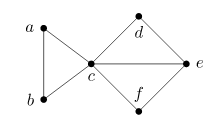
\includegraphics[width=.45\textwidth]{hw8_graphic2}
            \end{center}

            We need to find the number of valid combination of trees in this graph. Isolating each triangle into three sections. In the square portion, we have 8 valid tree, $(3)(8) = 24$ possible trees, resulting in 6 possible spanning trees.

        \end{enumerate}
	
	
	
		
\end{document}
